\documentclass[12pt, oneside, titlepage]{article}   	% use "amsart" instead of "article" for AMSLaTeX format

\usepackage{graphicx}
\graphicspath{ {\string} }
\usepackage{subcaption}

%%%%%%%%%%%%%%%%%%%%%%%%%%%%%%%%%%%%%%%%%%%%%%%%%%%%
% set up packages
%%%%%%%%%%%%%%%%%%%%%%%%%%%%%%%%%%%%%%%%%%%%%%%%%%%%
\usepackage{geometry}                
\usepackage{textcomp}                
\usepackage{amsmath}                
\usepackage{graphicx}                
\usepackage{amssymb}                
\usepackage{fancyhdr}                
\usepackage{subcaption}                
\usepackage{bm}                
\usepackage{tabularx}                

\usepackage{lineno}
% package for comments
\usepackage{soul}

\usepackage[breaklinks=true]{hyperref}

\usepackage[superscript,noadjust]{cite} % puts dash in citations to abbreviate
\usepackage [autostyle, english = american]{csquotes} % sets US-style quotes

\usepackage{etoolbox} % block quotes

\usepackage{float}
\usepackage{color}

\usepackage{pgf}
\usepackage{tikz}
\usepackage{eqnarray}

\usepackage{listings} % code blocks
\usepackage{setspace}

\usepackage{lscape}

% tikz background
\usetikzlibrary{backgrounds, fit}


\usepackage{natbib}
%\bibliographystyle{abbrvnat}
\setcitestyle{authoryear,open={(},close={)}}

%%%%%%%%%%%%%%%%%%%%%%%%%%%%%%%%%%%%%%%%%%%%%%%%%%%%
% call packages
%%%%%%%%%%%%%%%%%%%%%%%%%%%%%%%%%%%%%%%%%%%%%%%%%%%%	
\geometry{letterpaper, marginparwidth=60pt} % sets up geometry              		
\linenumbers % adds line numbers 
\MakeOuterQuote{"} % sets quote style
\doublespacing % setspace

%%%%%%%%%%%%%%%%%%%%%%%%%%%%%%%%%%%%%%%%%%%%%%%%%%%%
% patches with etoolbox 
%%%%%%%%%%%%%%%%%%%%%%%%%%%%%%%%%%%%%%%%%%%%%%%%%%%%	
% block quotes
\AtBeginEnvironment{quote}{\small}

% linenumbers
\makeatletter
\patchcmd{\@startsection}{\@ifstar}{\nolinenumbers\@ifstar}{}{}
\patchcmd{\@xsect}{\ignorespaces}{\linenumbers\ignorespaces}{}{}
\makeatother

%%%%%%%%%%%%%%%%%%%%%%%%%%%%%%%%%%%%%%%%%%%%%%%%%%%%
% tikzlibrary modifications
%%%%%%%%%%%%%%%%%%%%%%%%%%%%%%%%%%%%%%%%%%%%%%%%%%%%	
\usetikzlibrary{fit}
\usetikzlibrary{positioning}
\usetikzlibrary{arrows}
\usetikzlibrary{automata}

%%%%%%%%%%%%%%%%%%%%%%%%%%%%%%%%%%%%%%%%%%%%%%%%%%%%
% page formatting; exact 1 in margins
%%%%%%%%%%%%%%%%%%%%%%%%%%%%%%%%%%%%%%%%%%%%%%%%%%%%
\pagestyle{plain}                                                     

\setlength{\textwidth}{6.5in}    
\setlength{\oddsidemargin}{0in}
\setlength{\evensidemargin}{0in}
\setlength{\textheight}{8.5in}
\setlength{\topmargin}{0in}
\setlength{\headheight}{0in}
\setlength{\headsep}{0in}
\setlength{\footskip}{.5in}

%%%%%%%%%%%%%%%%%%%%%%%%%%%%%%%%%%%%%%%%%%%%%%%%%%%%
% defining code blocks using listings package
%%%%%%%%%%%%%%%%%%%%%%%%%%%%%%%%%%%%%%%%%%%%%%%%%%%%

\definecolor{dkgreen}{rgb}{0,0.6,0}
\definecolor{gray}{rgb}{0.5,0.5,0.5}
\definecolor{mauve}{rgb}{0.58,0,0.82}

\lstset{frame=tb,
  language=R,
  aboveskip=3mm,
  belowskip=3mm,
  showstringspaces=false,
  columns=flexible,
  basicstyle={\small\ttfamily},
  numbers=none,
  numberstyle=\tiny\color{gray},
 % keywordstyle=\color{blue},
  commentstyle=\color{dkgreen},
  stringstyle=\color{mauve},
  breaklines=true,
  breakatwhitespace=true,
  tabsize=3,
  otherkeywords={0,1,2,3,4,5,6,7,8,9},
  deletekeywords={data,frame,length,as,character,dunif,ps},
}

%%%%%%%%%%%%%%%%%%%%%%%%%%%%%%%%%%%%%%%%%%%%%%%%%%%%
%%%%%%%%%%%%%%%%%%%%%%%%%%%%%%%%%%%%%%%%%%%%%%%%%%%%
% begin document
%%%%%%%%%%%%%%%%%%%%%%%%%%%%%%%%%%%%%%%%%%%%%%%%%%%%
%%%%%%%%%%%%%%%%%%%%%%%%%%%%%%%%%%%%%%%%%%%%%%%%%%%%

\begin{document}

Last updated: \today

Seed banks present a challenge for models of plant population demography. Individual seeds can not be tracked and it is likely that there is greater uncertainty associated with seed bank vital rates. Ecologists have turned to various methods to assess survival and germination from the seed bank, including experimental burials and seed addition experiments.


The models below represent the joint likelihood for data from the seed bag experiments. All data from seed bags and viability trials is in the form of binomial trials: we have counts of seeds at the start and end of an experimental window of time. All models for the parameters $\theta_1, \theta_2, \theta_3, \theta_4, \theta_5$ have the same structure for seeds in bag $i$ in year $j$ in population $k$. If the number of seeds starting the trial (trials) is $n_{ijk}$ and the number of seeds at the end of the trial (successes) is $y_{ijk}$, we write a model that has a population-level mean and year-level means drawn from the population-level distribution. The probability of success for each bag is drawn from this year- and population-level distribution:

I compared convergence diagnostics (R-hat, effective sample size) for centered and non-centered parameterizations of the model. Here, I use the centered parameterization because this led to improved convergence. In each model, we obtain the population-level posterior distribution probability of success (the $\theta$s) by marginalizing across years and taking the inverse logit.

The seed bank experiments might used to obtain age-specific survival and recruitment terms. So the terms could be survival to month 3 (equal to age-specific survival at midpoint), germination at month 3, survival from month 3 to month 12 (equal to age-specific survival at midpoint), germination at month 15, survival from month 15 to 24, germination at month 27, survival from month 27 to 36. There are some errors in the data still, need to look at those. For germination there is no clear pattern to germination, either for individual sites or across sites. There are monotonic increases, monotonic decreases, and nonmonotonic patterns. Might also help to look at viability across age. 

The seed pot experiments seem like they would be amenable to the kind of functions fit in the paper by Rees and Long. In those cases there are only 3 time points which would limit the application of the empirical seedling recruitment curves. But perhaps overlaying them per population would allow us to figure out whether there is consistency across years or whether particular cohorts follow different curves, and how this varies in space?

I will estimate survival/mortality rates at 4 time points (0-3 months, 3-12 months, 15-24 months, 27-36 months), and germination at 3 time points (3 months, 15 months, 27 months). This will allow me to figure out what kind of model (cf Rees and Long) might be most appropriate for the data, especially for the emergence data from the seed pot trials. 

\singlespace

\begin{center}
\captionof{table}{ Summary of models in Rees and Long (1993). } \label{tab:title2} 
 \begin{tabularx}{\linewidth}{l X} 
 \hline
 \hline
\multicolumn{1}{ c }{ Model } & 
\multicolumn{1}{ c }{ Description } \\
 \hline
 %%%% VIABILITY TRIALS
% \multicolumn{2}{ l }{ \sc{Viability trials }} \\

  Exponential & \dots \\
 
  Compound exponential & \dots \\

   Weibull & \dots  \\
  
  Log logistic & \dots \\

  \hline
\end{tabularx}
\end{center}

\doublespace

I've now re-read Rees and Long (1993) and I think that's not the correct approach for the seed bag data. They present an analysis of recruited seedlings, fitting distributions to 5 years of data on emerged seedlings.

Instead, I think it would be useful to look at models for litter decomposition. I read Olson (1963) and Cornwell et al. (2014), which both present logic for analyzing litter decomposition experiments. Cornwell et al. (2014) have a series of functions in Table 1 that could serve as "process models". The approach I'm going to try is to use a sampling model that represents the binomial experiment (seeds in seed bags) and a process model that represents the decay of survival probability. 

We start with
%
\begin{align}
  \begin{split}
y_{it} &\sim \mathrm{binomial}(n_i, \theta) 
\\ \theta & \sim \mathrm{beta}(1,1)
  \end{split}
\end{align}
% 
to say that the observations of the number of seeds counted in bag $i$ at time $t$ are represented as $y_{it}$ drawn from a binomial distribution. In this case, $n_i$ is the number of trials, the number of seeds starting the experiment; $y_{it}$ is the number of successes, the number of seeds remaining. The $\theta$ is the probability of success on a single trial.
%
\begin{align}
  \begin{split}
[\theta | \bm{y}, \bm{n} ] \propto \mathrm{binomial}(y_{it} | n_i, \theta) \mathrm{beta}(\theta | 1,1)
  \end{split}
\end{align}
%

We then have sampling variability that is implicit in the binomial. There are thus two sources of uncertainty. Uncertainty arising from sampling and uncertainty arising because of \dots. 

The case where each bag has its own mean survival at each time, acknowledging variation among bags:
%
\begin{align}
  \begin{split}
y_{it} &\sim \mathrm{binomial}(n_i, \theta_{it}) 
\\ \theta_{it} & \sim \mathrm{beta}(\alpha,\beta)
  \end{split}
\end{align}
% 
Giving the following :
%
\begin{align}
  \begin{split}
[\bm{\theta}, \alpha, \beta | \bm{y}, \bm{n} ] & \propto \mathrm{binomial}(y_{it} | n_i, \theta_{it}) \mathrm{beta}(\theta _{it}| \alpha, \beta) 
\\ & \mathrm{gamma}( \alpha | 0.001, 0.001) \mathrm{gamma}( \beta | 0.001, 0.001)
  \end{split}
\end{align}
%
We now want to model the process "change in being intact with time" as 
%
\begin{align}
  \begin{split}
g(k,t_i) = \exp(-k t_i)
  \end{split}
\end{align}
% 
This deterministic model represents the average proportion of seeds that are expected to be intact as a function of time under a negative exponential process. The function $g(k,t_i)$ is the overall mean probability of being intact at time $t_i$. This is the mean of the beta distribution; the variance is the variation in probability of being intact at time $t_i$ that arises from differences among time. The uncertainty that arises from sampling - which we can estimate because of replication - is distinct from this process variance. I think the process variance is all effects that create variation beyond the seed age, as represented with a negative exponential function.

The next problem is that the process is not simply one of decay, decomposition, or mortality. Instead, there are annual events interspersed into this, namely germination. In this way I think the situation resembles the complement of case 2 in Olson (1963). Modeling germination and survival jointly would account for the full data. Here's one idea:
%
\begin{align}
  \begin{split}
h_1(k,t_1) & = \exp(-k t_1) \\
h_2(k,t_1) & = g_1  \exp(-k t_1) \\
h_3(k,t_2) & = (1-g_1)  \exp(-k t_2) \\
h_4(k,t_3) & = (1-g_1)  \exp(-k t_3) \\
h_5(k,t_3) & = (1-g_1) (g_2)  \exp(-k t_3) \\
h_6(k,t_4) & = (1-g_1) (1-g_2)  \exp(-k t_4) \\
h_7(k,t_5) & = (1-g_1) (1-g_2)  \exp(-k t_5) \\
h_8(k,t_5) & = (1-g_1) (1-g_2) g_3 \exp(-k t_5) \\
h_9(k,t_6) & = (1-g_1) (1-g_2) (1-g_3) \exp(-k t_6) \\
  \end{split}
\end{align}
%

Perhaps it would be productive to break the probability into two processes, one accounting for mortality and another accounting for decay. The one accounting for mortality would follow one of the following processes. First, we consider a negative exponential mortality trajectory.
%
\begin{align}
  \begin{split}
g(k,t_i) = \exp(-k t_i)
  \end{split}
\end{align}

Then, we consider a continuous exponential mortality trajectory:
%
\begin{align}
  \begin{split}
g(a,b,t_i) = \frac{1}{(1+bt_i)^a}
  \end{split}
\end{align}
% 

Then, we consider a mortality trajectory for Weibull residence times:
%
\begin{align}
  \begin{split}
g(\alpha,\beta,t_i) = \exp-(\frac{t_i}{\beta})^\alpha
  \end{split}
\end{align}

The mortality process would be multiplied with the process "change in removal from population with age due to germination", represented as
%
\begin{align}
  \begin{split}
h_1(\bm{g}) & = 1 \\
h_2(\bm{g}) & = g_1 \\
h_3(\bm{g}) & = (1-g_1) \\
h_4(\bm{g}) & = (1-g_1) \\
h_5(\bm{g}) & = (1-g_1) g_2 \\
h_6(\bm{g}) & = (1-g_1) (1- g_2) \\
h_7(\bm{g}) & = (1-g_1) (1- g_2) \\
h_8(\bm{g}) & = (1-g_1) (1- g_2) g_3 \\
h_9(\bm{g}) & = (1-g_1) (1- g_2) (1-g_3) \\
  \end{split}
\end{align}
% 

In turn we would consider models that combine age-dependent and -independent germination functions and mortality functions. The table below shows the models we considered, the parameters, and the number of parameters for each model. The product of the mortality and germination process is a deterministic function that equals the average proportion of seeds that are expected to be intact or germinated. This average proportion is the mean of a beta distribution with process variance that captures variation beyond the effect of seed age on mortality as represented with a mortality process and germination.  We might also consider a germination process where germination is randomly distributed and independent for each bag?

\singlespace

\begin{center}
\captionof{table}{ Seed bag dataset models } \label{tab:title2} 
 \begin{tabularx}{\linewidth}{l c c c c} 
 \hline
 \hline
 \multicolumn{1}{ c }{ Model } & 
\multicolumn{1}{ c }{ Mortality process } & 
\multicolumn{1}{ c }{ Germination process } & 
 \multicolumn{1}{ c }{ Parameters } & 
  \multicolumn{1}{ c }{ Parameter number }   \\
 \hline
 %%%% VIABILITY TRIALS
% \multicolumn{2}{ l }{ \sc{Viability trials }} \\

 A1 & Negative exponential & Constant & $k,g$ & 2 \\

 A2 & Negative exponential & Age-dependent & $k,g_{1-3}$ & 4 \\
 
  B1 &  Compound exponential & Constant & $a,b,g$ & 3  \\

  B2 &  Compound exponential & Age-dependent & $a,b,g_{1-3}$ & 5\\

  C1 &   Weibull residence time & Constant & $\alpha,\beta,g$ & 3 \\

  C2 &   Weibull residence time & Age-dependent & $\alpha,\beta,g_{1-3}$ & 5 \\
  
  \hline
\end{tabularx}
\end{center}

\doublespace

The following equations correspond to the full conditional distributions for models at the first time point. Subsequent models incorporate germination in the function $m(\dots,\sigma^2)$. Specifically, the mean is the product of the mortality up to time $t_i$, represented by $g(\dots)$, germination up to time $t_i$, represented by $h(\dots)$. We will use the information from the seed bag experiments to determine whether there is an appropriate mortality process with which to model the recruitment data from the seed pots. What I would like to do with this is get a mortality and germination process that's appropriate for these sites and use the posterior for the parameters in that process as informed priors to model the seed recruitment from the seed pots. 

The base assumption is often that seed mortality proceeds at a constant, absolute rate. Although this assumption has repeatedly been challenged (Lonsdale 1988, Rees and Long 1993) there remain limited assessments for how appropriate it is. A negative exponential model corresponds to the decay of radioactive isotopes. As described in Cornwell and Weedon (2014), this model has a constant decay parameter $k$ that implies the decaying material be treated as a homogeneous mass with each seed having an equal probability of mortality throughout time. But we know that seeds exhibit phenotypic variation in dormancy-related traits. The negative exponential decay model may be appropriate if seed survival is random in time and largely unrelated to seed characteristics.

The continuous exponential model is one in which seed mortality is described by a continuous quality distribution. 

The Weibull residence time model represents the seed pool as a distribution of survival times. Parameter alpha controls the shape of the decomposition trajectory and beta the rate of decomposition. This model can reduce to the exponential model when alpha is 1. If alpha is less than 1, the decomposition rate decreases through time. If alpha is greater than 1, the decomposition rate increases through time. 

Finally, we also consider the model proposed in Gremer and Venable (2014), namely one in which seed mortality is seasonal and age-dependent. 

\begin{align}
  \begin{split}
  %
  g(k,t_i) & = \exp(-k t_i) \\
  %
[ k , \alpha, \beta | \bm{y}, \bm{n} ] & \propto \mathrm{binomial}(y_{it} | n_i, \theta_{it}) \mathrm{beta}(\theta _{it}| m(g(k, t_i ), \sigma^2) ) 
%
\\ & \times \mathrm{gamma}( k | 0.001, 0.001) 
\\ & \times \mathrm{inverse\ gamma}( \sigma^2 | 0.001, 0.001) 
  \end{split}
\end{align}

\begin{align}
  \begin{split}
  %
  g(a,b,t_i) & = \frac{1}{(1+bt_i)^a}\\
  %
[ k , \alpha, \beta | \bm{y}, \bm{n} ] & \propto \mathrm{binomial}(y_{it} | n_i, \theta_{it}) \mathrm{beta}(\theta _{it}| m(g(a,b, t_i ), \sigma^2) ) 
%
\\ & \times \mathrm{gamma}( a | 0.001, 0.001) \mathrm{gamma}( b | 0.001, 0.001) 
\\ & \times \mathrm{inverse\ gamma}( \sigma^2 | 0.001, 0.001) 
  \end{split}
\end{align}

\begin{align}
  \begin{split}
g(\alpha,\beta,t_i) & = \exp-(\frac{t_i}{\beta})^\alpha \\
  %
[ k , \alpha, \beta | \bm{y}, \bm{n} ] & \propto \mathrm{binomial}(y_{it} | n_i, \theta_{it}) \mathrm{beta}(\theta _{it}| m(g(\alpha,\beta, t_i ) , \sigma^2) ) 
%
\\ & \times \mathrm{gamma}( \alpha | 0.001, 0.001) \times \mathrm{gamma}( \beta | 0.001, 0.001) 
\\ & \times \mathrm{inverse\ gamma}( \sigma^2 | 0.001, 0.001) 
%
  \end{split}
\end{align}



\clearpage
\newpage

\subsection*{Identifiability within years}
%%%%%%%%%%%%%%%%%%%%%%%%%%%%%%%%%%%%%%%%%%%%%%%%%%%%
% DIRECTED ACYCLIC GRAPHS FOR AGE 1 SEED BAGS
%%%%%%%%%%%%%%%%%%%%%%%%%%%%%%%%%%%%%%%%%%%%%%%%%%%%
\begin{figure}[h]%
\begin{subfigure}[c]{\textwidth}
   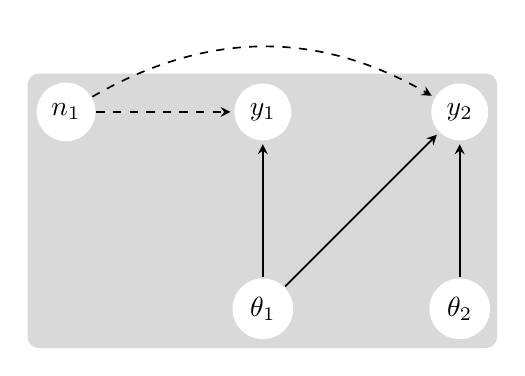
\begin{tikzpicture}[
            > = stealth, % arrow head style
            shorten > = 1pt, % don't touch arrow head to node
            auto,
            node distance = 2.5cm, % distance between nodes
            semithick % line style
        ]

        \tikzstyle{every state}=[
            draw = none,
            thick,
            fill = white,
            minimum size = 4mm
        ]F


	% data level
        \node[state] (Y) [] {$y_1$};
        \node[state] (N) [left of=Y] {$n_1$};
        \node[state] (Y2) [right of=Y] {$y_2$};
       
        \path[dashed,->] (N) edge node {} (Y);
        \path[dashed,->,bend left] (N) edge node {} (Y2);

         % parameters
         \node[state] (AB) [below of = Y] {$\theta_1$};
         \node[state] (AB2) [below of = Y2] {$\theta_2$};
                
         \path[->] (AB) edge node {} (Y);
         \path[->] (AB) edge node {} (Y2);
         \path[->] (AB2) edge node {} (Y2);
         
          \begin{scope}[on background layer]
   	  \node [fit=(N) (Y2) (AB), fill= gray!30, rounded corners, inner sep=.1cm] {};
          \end{scope}
          
  \end{tikzpicture}
  %
    \hspace{1cm}% NO SPACE!
  % BEGIN FIGURE 3
   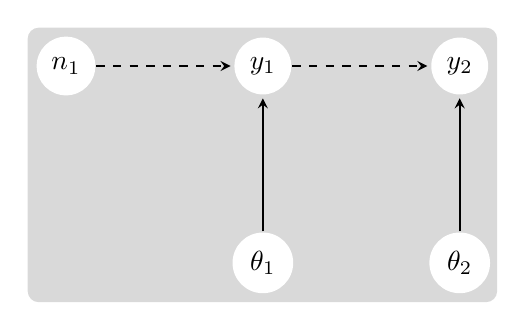
\begin{tikzpicture}[
              > = stealth, % arrow head style
            shorten > = 1pt, % don't touch arrow head to node
            auto,
            node distance = 2.5cm, % distance between nodes
            semithick % line style
        ]

        \tikzstyle{every state}=[
            draw = none,
            thick,
            fill = white,
            minimum size = 4mm
        ]F


	% data level
        \node[state] (Y) [] {$y_1$};
        \node[state] (N) [left of=Y] {$n_1$};
         \node[state] (Y2) [right of=Y] {$y_2$};
       
        \path[dashed,->] (N) edge node {} (Y);
        \path[dashed,->] (Y) edge node {} (Y2);

         % parameters
         \node[state] (AB) [below of = Y] {$\theta_1$};
         \node[state] (AB2) [below of = Y2] {$\theta_2$};
                
         \path[->] (AB) edge node {} (Y);
         \path[->] (AB2) edge node {} (Y2);
         
          \begin{scope}[on background layer]
   	  \node [fit=(N) (Y2) (AB), fill= gray!30, rounded corners, inner sep=.1cm] {};
          \end{scope}
                           
  \end{tikzpicture}
  %
\subcaption{Directed acyclic graphs for the hierarchical models for seed bag rates. Solid arrows depict the relationships among random variables, and dashed arrows depict the deterministic relationships.}
\end{subfigure}
\end{figure}
%
%%%%%%%%%%%%%%%%%%%%%%%%%%%%%%%%%%%%%%%%%%%%%%%%%%%%
% POSTERIOR AND JOINT DISTRIBUTIONS FOR AGE 1 SEED BAGS
%%%%%%%%%%%%%%%%%%%%%%%%%%%%%%%%%%%%%%%%%%%%%%%%%%%%

% QUESTIONS
% do I need to include \bm{n} on the RHS of the conditional statement for the posterior?

\begin{align}
  \begin{split}
 [  \theta_1, \theta_2  | & \bm{y_1} , \bm{y_2} ] \propto 
   \mathrm{binomial} ( y_1 | n_1, \mathrm{logit}^{-1}( \alpha_1 ) )  
      \\ & \times \mathrm{binomial} ( y_2 | n_1, \mathrm{logit}^{-1}( \alpha_1 ) \times \mathrm{logit}^{-1}( \alpha_2 ) ) 
   \\ & \times \mathrm{normal} ( \alpha_1  | \mu_1, \sigma_1 ) \mathrm{normal} ( \alpha_2  | \mu_2, \sigma_2 )
  \\ & \times \mathrm{normal} ( \mu_1 | 0 , 1000 ) \textrm{half-normal} ( \sigma_1 | 0,1)
    \\ & \times \mathrm{normal} ( \mu_2 | 0 , 1000 ) \textrm{half-normal} ( \sigma_2 | 0,1).
  \end{split}
\end{align}
%
\begin{align}
  \begin{split}
 [  \theta_1, \theta_2  | & \bm{y_1} , \bm{y_2} ] \propto 
   \mathrm{binomial} ( y_1 | n_1, \mathrm{logit}^{-1}( \alpha_1 ) )
      \\ & \times  \mathrm{binomial} ( y_2 | y_1, \mathrm{logit}^{-1}( \alpha_2 ) ) 
   \\ & \times \mathrm{normal} ( \alpha_1  | \mu_1, \sigma_1 ) \mathrm{normal} ( \alpha_2  | \mu_2, \sigma_2 )
  \\ & \times \mathrm{normal} ( \mu_1 | 0 , 1000 ) \textrm{half-normal} ( \sigma_1 | 0,1)
    \\ & \times \mathrm{normal} ( \mu_2 | 0 , 1000 ) \textrm{half-normal} ( \sigma_2 | 0,1).
  \end{split}
\end{align}
%

\clearpage
\newpage


\subsection*{Identifiability across years}
%%%%%%%%%%%%%%%%%%%%%%%%%%%%%%%%%%%%%%%%%%%%%%%%%%%%
% DIRECTED ACYCLIC GRAPHS FOR AGE 1 SEED BAGS
%%%%%%%%%%%%%%%%%%%%%%%%%%%%%%%%%%%%%%%%%%%%%%%%%%%%
\begin{figure}[h]%
\begin{subfigure}[c]{\textwidth}
   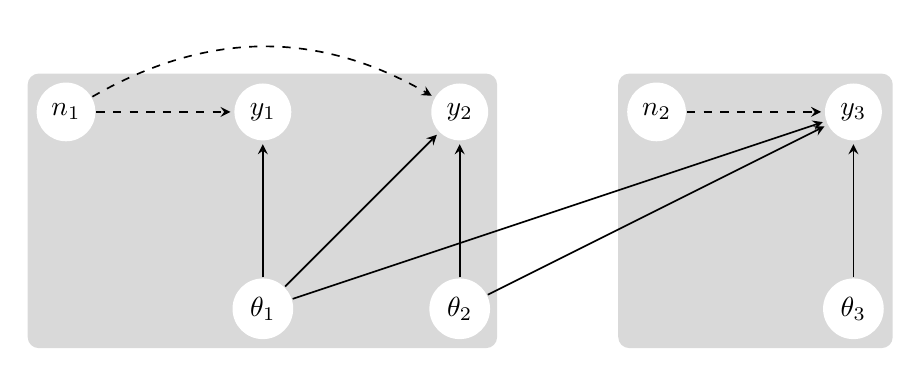
\begin{tikzpicture}[
            > = stealth, % arrow head style
            shorten > = 1pt, % don't touch arrow head to node
            auto,
            node distance = 2.5cm, % distance between nodes
            semithick % line style
        ]

        \tikzstyle{every state}=[
            draw = none,
            thick,
            fill = white,
            minimum size = 4mm
        ]F


	% data level
        \node[state] (Y) [] {$y_1$};
        \node[state] (N) [left of=Y] {$n_1$};
        \node[state] (Y2) [right of=Y] {$y_2$};
        \node[state] (N2) [right of=Y2] {$n_2$};
        \node[state] (Y3) [right of=N2] {$y_3$};
       
        \path[dashed,->] (N) edge node {} (Y);
        \path[dashed,->,bend left] (N) edge node {} (Y2);
        \path[dashed,->] (N2) edge node {} (Y3);

         % parameters
         \node[state] (AB) [below of = Y] {$\theta_1$};
         \node[state] (AB2) [below of = Y2] {$\theta_2$};
         \node[state] (AB3) [below of = Y3] {$\theta_3$};
                
         \path[->] (AB) edge node {} (Y);
         \path[->] (AB) edge node {} (Y2);
         \path[->] (AB2) edge node {} (Y2);
         \path[->] (AB) edge node {} (Y3);
         \path[->] (AB2) edge node {} (Y3);
         \path[->] (AB3) edge node {} (Y3);
         
          \begin{scope}[on background layer]
   	  \node [fit=(N) (Y2) (AB),fill=gray!30, rounded corners, inner sep=.1cm] {};
	  \node [fit=(N2) (Y3) (AB3),fill=gray!30, rounded corners, inner sep=.1cm] {};
          \end{scope}
          
  \end{tikzpicture} \\ \\ \\
   % BEGIN FIGURE 3
 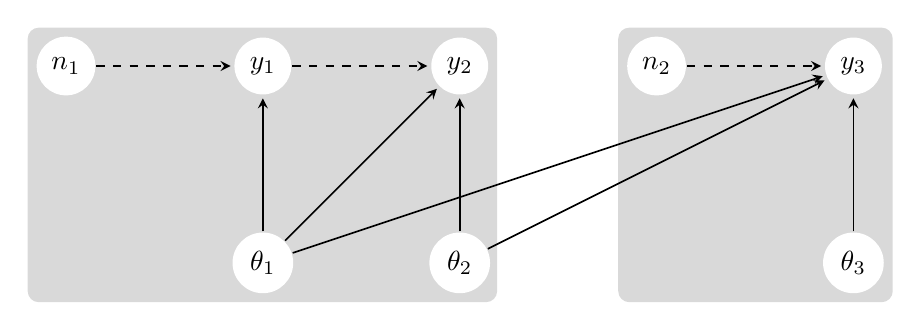
\begin{tikzpicture}[
            > = stealth, % arrow head style
            shorten > = 1pt, % don't touch arrow head to node
            auto,
            node distance = 2.5cm, % distance between nodes
            semithick % line style
        ]

        \tikzstyle{every state}=[
            draw = none,
            thick,
            fill = white,
            minimum size = 4mm
        ]F


	% data level
        \node[state] (Y) [] {$y_1$};
        \node[state] (N) [left of=Y] {$n_1$};
        \node[state] (Y2) [right of=Y] {$y_2$};
        \node[state] (N2) [right of=Y2] {$n_2$};
        \node[state] (Y3) [right of=N2] {$y_3$};
       
        \path[dashed,->] (N) edge node {} (Y);
        \path[dashed,->] (Y) edge node {} (Y2);
        \path[dashed,->] (N2) edge node {} (Y3);

         % parameters
         \node[state] (AB) [below of = Y] {$\theta_1$};
         \node[state] (AB2) [below of = Y2] {$\theta_2$};
         \node[state] (AB3) [below of = Y3] {$\theta_3$};
                
         \path[->] (AB) edge node {} (Y);
         \path[->] (AB) edge node {} (Y2);
         \path[->] (AB2) edge node {} (Y2);
         \path[->] (AB) edge node {} (Y3);
         \path[->] (AB2) edge node {} (Y3);
         \path[->] (AB3) edge node {} (Y3);
         
          \begin{scope}[on background layer]
   	  \node [fit=(N) (Y2) (AB),fill=gray!30, rounded corners, inner sep=.1cm] {};
	  \node [fit=(N2) (Y3) (AB3),fill=gray!30, rounded corners, inner sep=.1cm] {};
          \end{scope}
          
  \end{tikzpicture}
  %
\subcaption{Directed acyclic graphs for the hierarchical models for seed bag rates. Solid arrows depict the relationships among random variables, and dashed arrows depict the deterministic relationships.}
\end{subfigure}
\end{figure}
%
%%%%%%%%%%%%%%%%%%%%%%%%%%%%%%%%%%%%%%%%%%%%%%%%%%%%
% POSTERIOR AND JOINT DISTRIBUTIONS FOR AGE 1 SEED BAGS
%%%%%%%%%%%%%%%%%%%%%%%%%%%%%%%%%%%%%%%%%%%%%%%%%%%%

% QUESTIONS
% do I need to include \bm{n} on the RHS of the conditional statement for the posterior?

\begin{align}
  \begin{split}
 [  \theta_1, \theta_2  | & \bm{y_1} , \bm{y_2} ] \propto 
   \mathrm{binomial} ( y_1 | n_1, \mathrm{logit}^{-1}( \alpha_1 ) )  
      \\ & \times \mathrm{binomial} ( y_2 | n_1, \mathrm{logit}^{-1}( \alpha_1 ) \times \mathrm{logit}^{-1}( \alpha_2 ) ) 
   \\ & \times \mathrm{normal} ( \alpha_1  | \mu_1, \sigma_1 ) \mathrm{normal} ( \alpha_2  | \mu_2, \sigma_2 )
  \\ & \times \mathrm{normal} ( \mu_1 | 0 , 1000 ) \textrm{half-normal} ( \sigma_1 | 0,1)
    \\ & \times \mathrm{normal} ( \mu_2 | 0 , 1000 ) \textrm{half-normal} ( \sigma_2 | 0,1).
  \end{split}
\end{align}
%
\begin{align}
  \begin{split}
 [  \theta_1, \theta_2  | & \bm{y_1} , \bm{y_2} ] \propto 
   \mathrm{binomial} ( y_1 | n_1, \mathrm{logit}^{-1}( \alpha_1 ) )
      \\ & \times  \mathrm{binomial} ( y_2 | y_1, \mathrm{logit}^{-1}( \alpha_2 ) ) 
   \\ & \times \mathrm{normal} ( \alpha_1  | \mu_1, \sigma_1 ) \mathrm{normal} ( \alpha_2  | \mu_2, \sigma_2 )
  \\ & \times \mathrm{normal} ( \mu_1 | 0 , 1000 ) \textrm{half-normal} ( \sigma_1 | 0,1)
    \\ & \times \mathrm{normal} ( \mu_2 | 0 , 1000 ) \textrm{half-normal} ( \sigma_2 | 0,1).
  \end{split}
\end{align}
%

\clearpage
\newpage

\subsection*{Exponential decay}
%%%%%%%%%%%%%%%%%%%%%%%%%%%%%%%%%%%%%%%%%%%%%%%%%%%%
% DIRECTED ACYCLIC GRAPHS FOR AGE 1 SEED BAGS
%%%%%%%%%%%%%%%%%%%%%%%%%%%%%%%%%%%%%%%%%%%%%%%%%%%%
\begin{figure}[h]%
\begin{subfigure}[c]{\textwidth}
   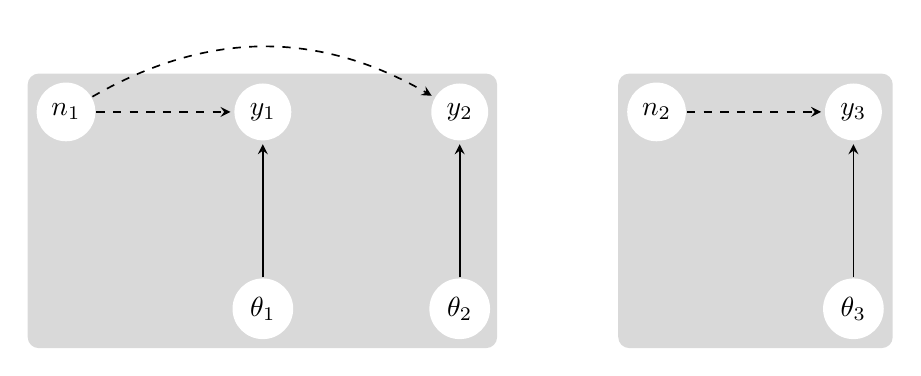
\begin{tikzpicture}[
            > = stealth, % arrow head style
            shorten > = 1pt, % don't touch arrow head to node
            auto,
            node distance = 2.5cm, % distance between nodes
            semithick % line style
        ]

        \tikzstyle{every state}=[
            draw = none,
            thick,
            fill = white,
            minimum size = 4mm
        ]F


	% data level
        \node[state] (Y) [] {$y_1$};
        \node[state] (N) [left of=Y] {$n_1$};
        \node[state] (Y2) [right of=Y] {$y_2$};
        \node[state] (N2) [right of=Y2] {$n_2$};
        \node[state] (Y3) [right of=N2] {$y_3$};
       
        \path[dashed,->] (N) edge node {} (Y);
        \path[dashed,->,bend left] (N) edge node {} (Y2);
        \path[dashed,->] (N2) edge node {} (Y3);

         % parameters
         \node[state] (AB) [below of = Y] {$\theta_1$};
         \node[state] (AB2) [below of = Y2] {$\theta_2$};
         \node[state] (AB3) [below of = Y3] {$\theta_3$};
                
         \path[->] (AB) edge node {} (Y);
         \path[->] (AB2) edge node {} (Y2);
         \path[->] (AB3) edge node {} (Y3);
         
          \begin{scope}[on background layer]
   	  \node [fit=(N) (Y2) (AB),fill=gray!30, rounded corners, inner sep=.1cm] {};
	  \node [fit=(N2) (Y3) (AB3),fill=gray!30, rounded corners, inner sep=.1cm] {};
          \end{scope}
          
  \end{tikzpicture} \\ \\ \\
   % BEGIN FIGURE 3
 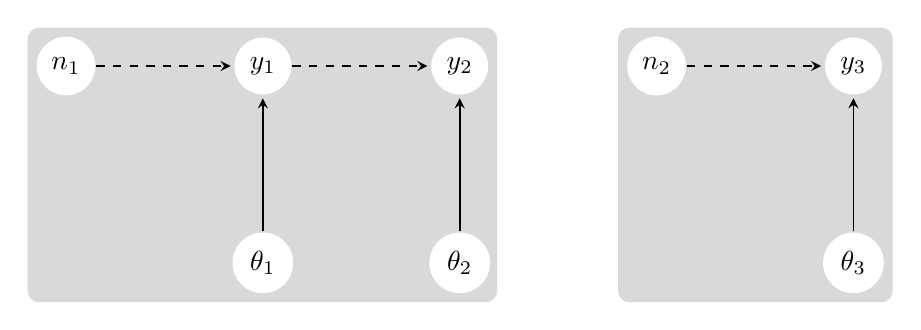
\begin{tikzpicture}[
            > = stealth, % arrow head style
            shorten > = 1pt, % don't touch arrow head to node
            auto,
            node distance = 2.5cm, % distance between nodes
            semithick % line style
        ]

        \tikzstyle{every state}=[
            draw = none,
            thick,
            fill = white,
            minimum size = 4mm
        ]F


	% data level
        \node[state] (Y) [] {$y_1$};
        \node[state] (N) [left of=Y] {$n_1$};
        \node[state] (Y2) [right of=Y] {$y_2$};
        \node[state] (N2) [right of=Y2] {$n_2$};
        \node[state] (Y3) [right of=N2] {$y_3$};
       
        \path[dashed,->] (N) edge node {} (Y);
        \path[dashed,->] (Y) edge node {} (Y2);
        \path[dashed,->] (N2) edge node {} (Y3);

         % parameters
         \node[state] (AB) [below of = Y] {$\theta_1$};
         \node[state] (AB2) [below of = Y2] {$\theta_2$};
         \node[state] (AB3) [below of = Y3] {$\theta_3$};
                
         \path[->] (AB) edge node {} (Y);
         \path[->] (AB2) edge node {} (Y2);
         \path[->] (AB3) edge node {} (Y3);
         
          \begin{scope}[on background layer]
   	  \node [fit=(N) (Y2) (AB),fill=gray!30, rounded corners, inner sep=.1cm] {};
	  \node [fit=(N2) (Y3) (AB3),fill=gray!30, rounded corners, inner sep=.1cm] {};
          \end{scope}
          
  \end{tikzpicture}
  %
\subcaption{Directed acyclic graphs for the hierarchical models for seed bag rates. Solid arrows depict the relationships among random variables, and dashed arrows depict the deterministic relationships.}
\end{subfigure}
\end{figure}

\end{document}
